\chapter{System Architecture}

\section{Technologies Used}
\subsection{Platform and Technologies - Application Server}
\begin{itemize}
  \item Implemented using Ruby on Rails web framework \cite{Ruby}
  \item Database is designed using MySQL
  \item GCM Server
\end{itemize}

\subsection{Application Design}

\begin{itemize}
\item Android Platform with Android Studio 1.1.0 \cite{Intro42:online}
\item Database is designed using SQLite.
\item Using Volley Libraries for asynchronous task communication to the network server \cite{Andro34:online}
\item Android 5.0.1 Minimum SDK build tool and Platform tool with APIs level 21 or above support
\item GCM Client
\end{itemize}

\section{System Flow}

Following Diagram depicts the entire System Flow.
\begin{figure}[H]
    \centering
	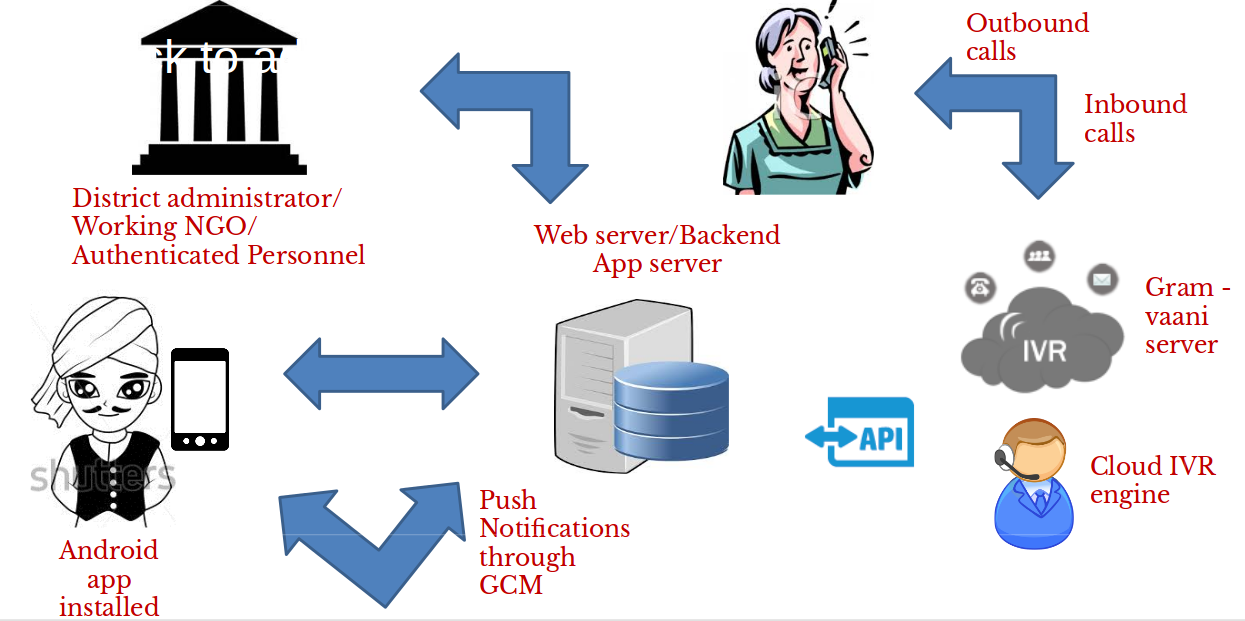
\includegraphics[width=0.8\textwidth]{Sysflow.png}
    \caption{System Flow}
    \label{fig:System Flow}
\end{figure}

\section{Use Case Diagram}
\begin{figure}[H]
    \centering
	\includegraphics[width=0.8\textwidth]{UseCaseDiagram.png}
    \caption{Use Case Diagram of Application User}
    \label{fig:Use Case Diagram of Application User}
\end{figure}

\section{Class Diagram}
\section{ERD Schema}
\section{Information flow}
Mobile Application is designed for the volunteers of the village. Along with, a portal is designed for the  NGOs/ Block or district officials for sending alerts to the volunteers of the community. Some volunteers from the community ( For instance, panchayat members, School teachers) will be chosen by the functioning NGO or block/ district administrator under which the community/ village falls. NGOs/ Block or district officials will give authorization to the selected volunteers from that community by registering them through the portal. After authorization, volunteers will be given an Android phone pre-loaded with the local governance application “ Gologo”. Credentials of volunteers will be authenticated on first time login in the application. After successful one time login, volunteers aid their local community people by exploring the app functionalities. Portal will be used to send survey alerts to the volunteers. Volunteers will receive alerts  on their mobile phones to further disperse it to the target people. Through this way, information will flow by the people and  among the people via following functionalities.

Following diagram depicts the functionalities provided to the app user.

\begin{figure}[H]
    \centering
	\includegraphics[width=10cm,height=10cm,keepaspectratio]{Workflowapp.png}
    \caption{Functionalities of Application User}
    \label{fig:Functionalities of Application User}
\end{figure}

Following Diagram depicts the flow of information through \hyperref[itm:launchsur]{Launch Survey Use Case} whcih is explained later.

\begin{figure}[H]
    \centering
	\includegraphics[width=0.9\textwidth]{launchsurvey1.png}
    \caption{Launch Survey Use Case}
    \label{fig:Launch Survey Use Case}
\end{figure}
